%! Author = lester
%! Date = 2026-09-14

% Preamble
\documentclass[%
 reprint,
%superscriptaddress,
%groupedaddress,
%unsortedaddress,
%runinaddress,
%frontmatterverbose,
%preprint,
%preprintnumbers,
nofootinbib,
%nobibnotes,
%bibnotes,
 amsmath,amssymb,
 aps,
%pra,
%prb,
%rmp,
%prstab,
%prstper,
floatfix,
]{revtex4-2}

% Packages
\usepackage{graphicx}% Include figure files
\usepackage{dcolumn}% Align table columns on decimal point
\usepackage{bm}% bold math
\usepackage{siunitx}
\usepackage{booktabs}
\usepackage{derivative}
\usepackage{amsmath}

%\usepackage[giveninits=true]{biblatex}
%\addbibresource{references.bib}

% Recommended options for physics papers:
\sisetup{
  separate-uncertainty = true, % Prints as (value ± uncertainty) unit instead of value(unc) unit
  multi-part-units = single    % Ensures units are not repeated, e.g., (1.23 ± 0.04) m instead of 1.23 m ± 0.04 m
}


\newcommand{\UVic}{\affiliation{Department of Physics and Astronomy, University of Victoria, Canada}}
\newcommand{\dif}{\mathop{}\!\mathrm{d}}

% Document
\begin{document}

% \preprint{APS/123-QED}

%\title{ \textcolor{red}{Fancy Science Paper}}
\title{Ferromagnetism}%

\author{Mark Lester}\UVic

\date{\today}% It is always \today, today,
             %  but any date may be explicitly specified

\begin{abstract}

%Presents the major aspects of the investigation and includes:
%1) the overall purpose of the lab;
%2) the basic design of the
%investigation;
%3) major findings or trends found;
%4) a summary of interpretations and conclusions.

    Ferromagnetic materials such as steel produce hysteresis curves when magnetised by an external magnetic field.
    This experiment aims to study the hysteresis effect by driving current through a steel toroid and plotting its
    magnetic response.
    Our results show that driving current up and down from a maximum of 2.0 Amps exhibited a closed loop hysteresis
    curve, where the integrated area was \qty{439.8}{\tesla\ampere\per\meter}.
    This quantity represented the work done per unit volume by the current.
    Despite residual magnetic field effects, the plot demonstrated a magnetic response which aligned with the
    ferromagnetic theory.
\end{abstract}


%\keywords{Suggested keywords}%Use showkeys class option if keyword
 %display desired
\maketitle

 %\tableofcontents
\section{Introduction}


%Presents a clear learning context and includes:
%1) the general scientific concept with the necessary background;
%2) primary goals and the specific scientific concept to be investigated;
%2) specific theory, experimental design and equations needed with fully defined quantities;
%3) any assumptions made or required;
%4) hypothesis to be investigated;
%5) references to supporting sources.

Applying a magnetic field across a ferromagnetic material changes its magnetic response.
In the case of steel, this response is characterised by a hysteresis curve, where ramping up the current produces a
different path compared to reversing the current.
In this experiment we aim to demonstrate the B-H hysteresis curve of a steel toroid by measuring the voltage in the 
coil as the current is adjusted up and down, as well as the magnetic induction.

The magnetic field strength, denoted as $H$, is found using the voltage and resistance of the coil.

\begin{equation}
            \label{eq:H}
    |\vec{H}| = H = \frac{N \cdot i}{L} = \frac{N}{2 \pi r} \frac{V}{R}
\end{equation}

Where, $N$ is the number of turns in the toroid, $i$ is the current (also may be calculated using Ohm's Law), $R$ is
the resistance of the coil, and $
r$ is the radius.

The work done per volume of the material may be found as

\begin{equation}
    \frac{W}{V} = \oint \vec{B} \cdot  d\vec{H} \label{eq:work}
\end{equation}

Where $W$ is the work done, $V$ is the volume of the material, $\vec{B}$ is the magnetic induction, and $d\vec{H}$ 
is the magnetic field strength element.

Magnetic susceptibility, $\chi$, is the quantity which describes how well the material aligns with the applied magnetic 
field, or how easily it is magnetised.
In ferromagnetic materials, this can be calculated using 

\begin{equation}
    B = \mu_0(1 + \chi) H\label{eq:chi}
\end{equation}

Where $\mu_0$ is the permeability of free space.

%Ref equation: Eqs.~\eqref{eq:norm_damp}, ~\eqref{eq:crit_damp}, and \eqref{eq:osc_damp}, respectively.
\section{Apparatus}\label{sec:apparatus}
%--------------------------------------------------

%Equipment: Vernier LabPro sensor interface, LabPro software, 4000 turn inductor, electrolytic capacitor, decade
%resistance box...

Equipment: Vernier LabPro sensor interface, LabPro software, toroid assembly, double-throw-double-pole commutator
switch, magnetic sensor, rheostat, leads, Wavetek LCR55 DMM\@.


\begin{figure}[htb]
    \centering
    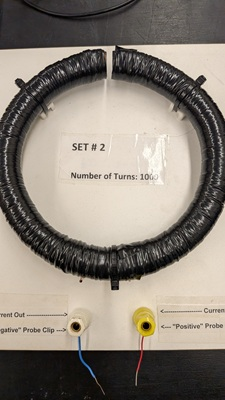
\includegraphics[width=\linewidth,height=0.35\textheight,keepaspectratio]{figs/toroid}
    \caption{Toroid of steel. Wrapped in copper wire.}
    \label{fig:toroid}
\end{figure}


\begin{figure}[htb]
    \centering
    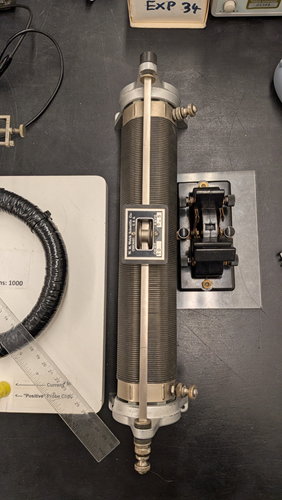
\includegraphics[width=\linewidth,height=0.35\textheight,keepaspectratio]{figs/rheostat}
    \caption{Rheostat}
    \label{fig:rheo}
\end{figure}
\section{Procedure}\label{sec:procedure}


%Presents the apparatus and procedure used and includes:
%1) a list of the apparatus;
%2) an apparatus diagram; 3) the technical details of the investigation in the procedure used to acquire data.
%Written in the past tense with specific terminology, this should allow others to replicate the experiment.


The experimental apparatus and procedure followed the standard method outlined in the University of Victoria PHYS 326
laboratory manual~\cite{phys326}.

Before any data was collected, the diameter of the toroid was measured using a 30cm ruler.
The diameter was determined from measuring the middle-middle of the shape in order to derive the total length, $L$.
The Hall sensor, which measures the magnetic field intensity, was positioned between the gap of the toroid seen in
Figure~\ref{fig:toroid}, and angled perpendicular to the incoming field lines.

The LoggerPro software was then sut up to measure the voltage across the coil as well as manual entries from the
Gaussmeter.
The Gaussmeter measurements were converted to units of Teslas.

A calculated column was used to determine $H$ using Eq.~\eqref{eq:H}.
A technique was employed in an attempt to demagnetise the metal sample.
First, the coil was energised up to 2.0 Amps to substantially polarise the material, then switched to a reverse
current of the same magnitude using the commutator switch to reverse the polarity.
This was repeated in 0.1 Amp increments all the way down to zero amps.
After four attempts of this technique, the lowest reading from the Gaussmeter was 11.3 G.

Starting from zero Amps, the data was collected in small intervals by entering in the digital voltage and Gaussmeter
readings into LoggerPro.
Once a maximum current of 2.0 Amps was reached, data was taken as current was reduced incrementally back down to zero.
At that point, the commutator switch was flipped to reverse the direction of current, and the process was repeated
to capture more data points to a maximum of 2.0 Amps.
Current was again reduced to zero where the data approximately closed the hysteresis curve.

\begin{table}[htbp]
    \caption{Experimental Parameters}
    \begin{tabular}{lrrr}
        \toprule
        {Quantity}           & {Reading}                \\
        \midrule
        $r$, Toroid radius   & \qty{82(5)}{\milli\meter} \\
        $N$, Number of turns & 1000                     \\
        $R$, Coil resistance & \qty{3.488(0.010)}{\ohm} \\
        \bottomrule
    \end{tabular}\label{tab:params}
\end{table}

Table~\ref{tab:params} provides a list of measurements taken.

The measurement uncertainty of $\pm 5$ millimeters was used to account for the uneven shape of the electrical tape
around the toroid and the ruler millimeter graduations.
The measurement uncertainty of resistance is taken from the DMM's spec sheet.
\section{Results}


%Presents the results of the procedure and includes:
%1) all data collected in tabular form if possible;
%2) all required graphs;
%3) all results in a logical sequence;
%4) objective observations;
%Note: all figures, tables and graphs required should include
%titles, labels, units and legends where appropriate.

%Present processed data, not raw data.

%The accepted value of $\gamma$ for dry air at room temperature ($\gamma = 1.40$) was taken from standard reference
%data~\cite{CRC}.

\begin{figure}[htb]
    \centering
    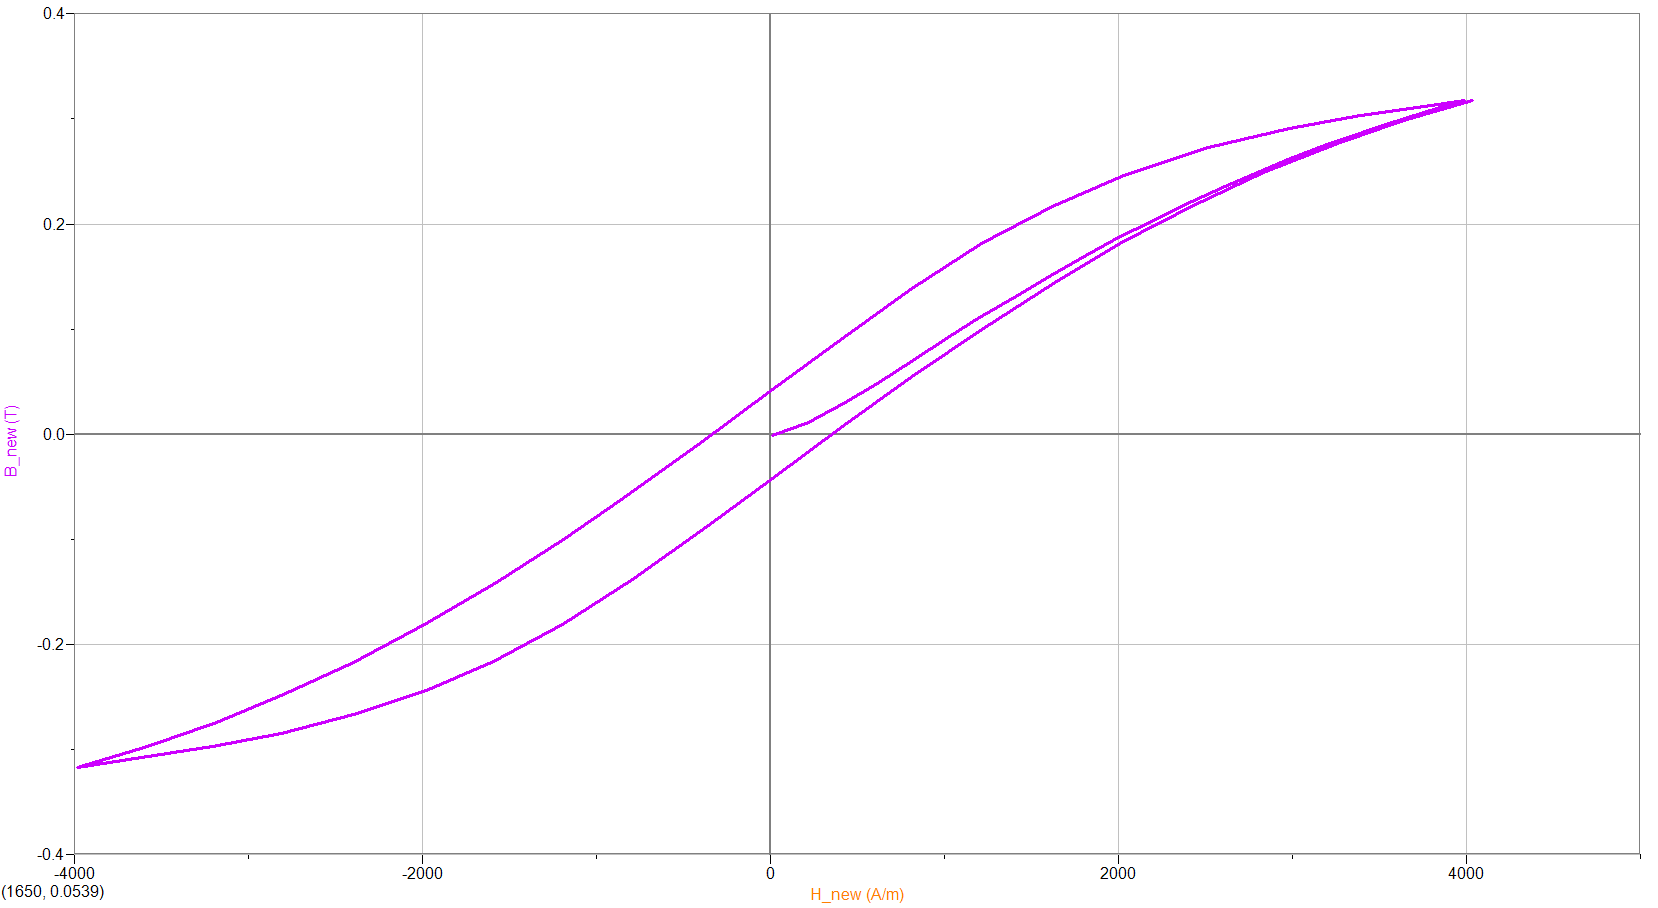
\includegraphics[width=\linewidth]{figs/hysteresis}
    \caption
    {The full magnetic response of the material from -2.0 A to + 2.0 A. The y-axis is $\vec{B}$, x-axis is $\vec{H}$}
    \label{fig:hysteresis}
\end{figure}

Figure~\ref{fig:hysteresis} shows the full data captured from the experiment.
The magnetic response was different depending on whether forward or reverse current was applied, and the which
direction it was incremented (towards 2.0 Amps or zero).

\begin{figure}[htb]
    \centering
    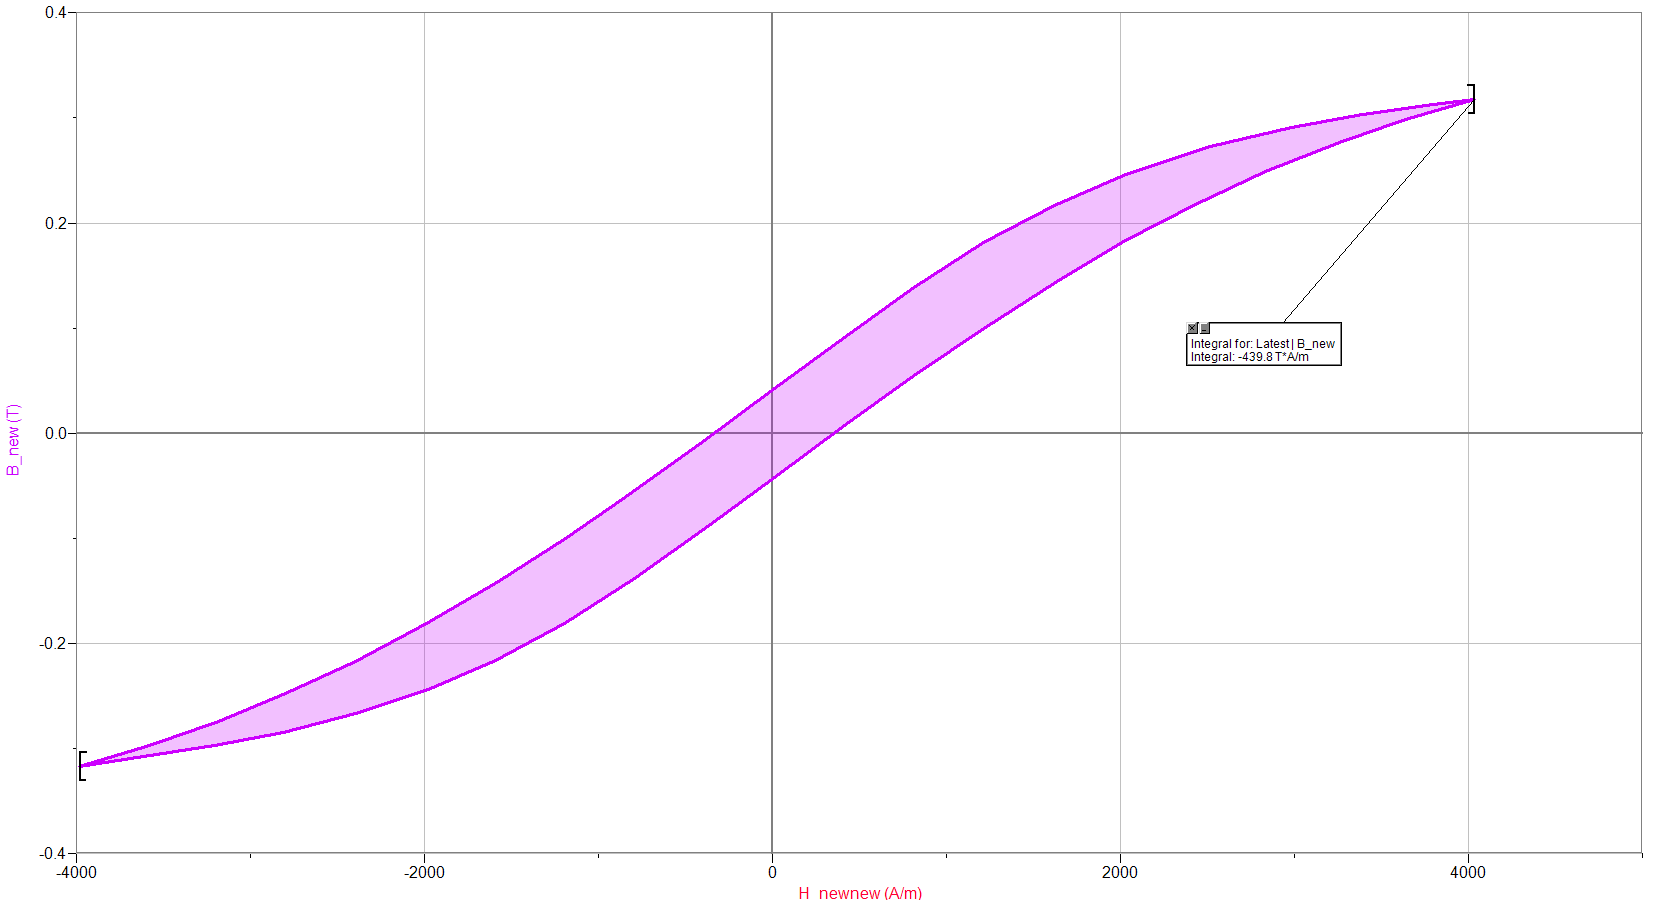
\includegraphics[width=\linewidth]{figs/integral}
    \caption{The integral of the closed loop was done with the LoggerPro software, minus the initial phase. Area
        = -439.8 T A/m.}
    \label{fig:integral}
\end{figure}

Integrating the closed loop as shown in Figure~\ref{fig:integral} produced an area of \qty{439.8}{\tesla\ampere\per\meter}.
From Eq.~\eqref{eq:work}, the area of enclosed by the curve is equal to the work done per volume.
The units from the plot are \qty{}{\tesla\ampere\per\meter}.
This is equivalent to \qty{}{\meter\kilogram\second} by performing dimensional analysis:

%\begin{align*}
%    \frac{\unit{\tesla\ampere}}{\unit{\meter}} &= \frac{\unit{\newton}}{\unit{\ampere\meter}}
%    \frac{\unit{\ampere}}{\unit{
%        \meter}} \\
%    &= \frac{\unit{\newton}}{\meter^2} \\
%    &= \frac{\unit{\newton\meter}}{\unit{\meter^3}} \\
%    &= \frac{\unit{\joule}}{\unit{\meter^3}} \quad \because \unit{\joule} = \unit{\newton\meter}
%\end{align*}


\begin{align*}
    \frac{\unit{\tesla\ampere}}{\unit{\meter}}
      &= \frac{\unit{\newton}}{\unit{\ampere\meter}}
         \cdot \frac{\unit{\ampere}}{\unit{\meter}} \\
      &= \frac{\unit{\newton}}{\unit{\meter\squared}} \\
      &= \frac{\unit{\newton\meter}}{\unit{\meter\cubed}} \\
      &= \frac{\unit{\joule}}{\unit{\meter\cubed}}
         && \because \unit{\joule} = \unit{\newton\meter}
\end{align*}


Now this can be expressed in meter-kilogram-second units.

\begin{align*}
    \frac{\unit{\joule}}{\unit{\meter}^3} &= \unit{\kilogram} \frac{\unit{\meter}^2}{\unit{\second}^2}
    \frac{1}{\unit{\meter}^3} \\
    &= \frac{\unit{\kilogram}}{\unit{\meter\second^2}}
\end{align*}

The value is unchanged, so this can be represented as \qty{439.8}{\kilogram\per\meter\second^2}.
This area represents the work done per unit volume by the current to magnetise the material throughout the whole
cycle.

The specific heat capacity of steel is \qty{420}{\joule\per\kilogram\per\celsius}.
Using the density of steel, \qty{7.8E3}{\kilogram\per\meter^3} we determine the temperature increase due the work done
throughout the whole cycle we perform the following
calculation:

\begin{align*}
    c &= \frac{W}{m \Delta T} \quad \text{specific heat}\\
    \implies \Delta T &= \frac{W}{V} \frac{1}{\rho c} \\
    &= (439.8) \frac{1}{(\qty{7.8E3}{}) (420)} \unit{\celsius} \\
    &= \qty{1.34E-4}{\celsius}
\end{align*}

\qty{1.34E-4}{\celsius} is the temperature increase if we assume all the work done is converted into Joule heating in the steel.
Since this is less than a tenth of a degree Celsius, this temperature increase would not be directly measurable
using a thermometer with a \qty{0.1}{\celsius} resolution.
Practical uses of measuring this temperature would be to protect sensitive electronic equipment.
Any measurable increase in temperature would indicate a large, perhaps unexpected current surge.
Alternatively, since heat accumulates, a noticeable temperature increase would give an
indication that the material had undergone multiple cycles.

\begin{figure}[htb]
    \centering
    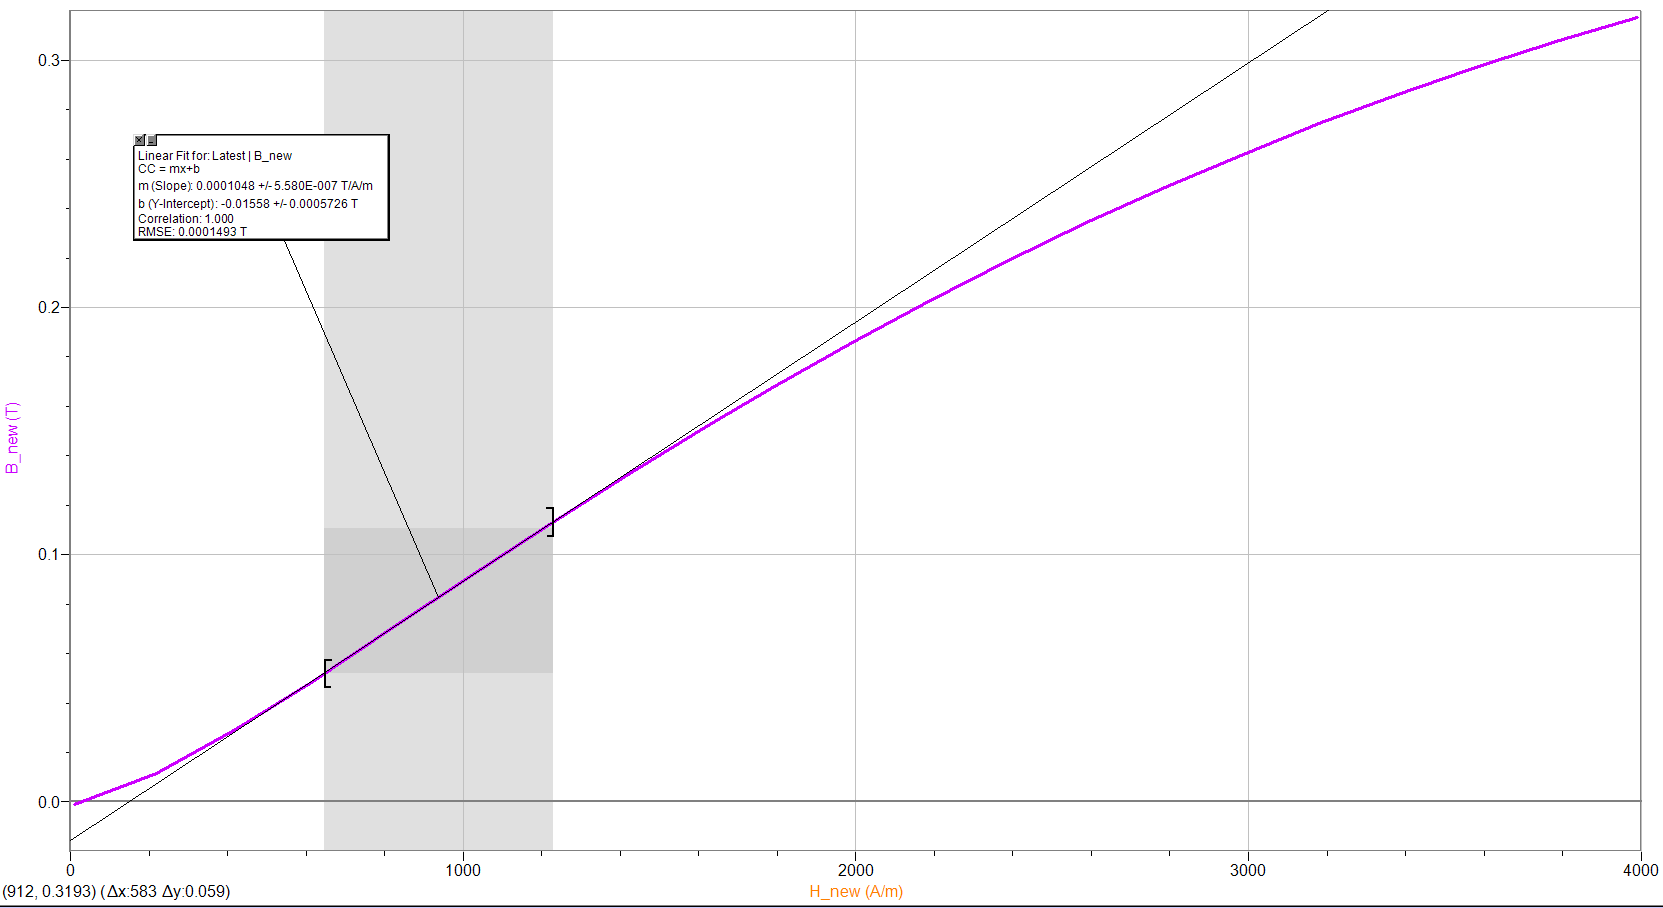
\includegraphics[width=\linewidth]{figs/slope}
    \caption{The maximum slope found during the initial phase. Slope =
    $\qty{104.8(0.56)e-6}{\tesla\meter\per\ampere}$}\label{fig:slope}
\end{figure}

By examining the maximum slope of the initial phase as in Figure~\ref{fig:slope}, we can determine the maximum susceptibility of
the
material via
Eq.~\eqref{eq:chi}.

\begin{align*}
    B &= \mu_0(1 + \chi) H \\
    \implies \chi &= \frac{B}{\mu_0 H} - 1 \\
    &= \frac{\qty{104.80(0.56)E-6}{}}{(4 \pi \times 10^{-7})} - 1 \\
    &= \qty{82.40(0.45)}{}
\end{align*}

This value, magnetic susceptibility, represents how strongly the material aligns with the applied magnetic field.
Since this was derived from the maximum slope, this is the maximum susceptibility of the material.




%\begin{table}[htbp]
%    \caption{Final results}
%    \resizebox{\columnwidth}{!}{%
%        \begin{tabular}{llccc}
%            \toprule
%            Gas                 & Experimental  & Accepted & Error (\%) & Consistency \\
%            \midrule
%            Air                 & 1.369+/-0.064 & 1.402    & 2.35       & PASS        \\
%            Argon               & 1.625+/-0.076 & 1.664    & 2.37       & PASS        \\
%            CO\textsubscript{2} & 1.278+/-0.060 & 1.293    & 1.15       & PASS        \\
%            \bottomrule
%        \end{tabular}
%    }
%    \label{tab:results}
%\end{table}

% Transposed version
%\begin{table}[htbp]
%    \caption{Final results}
%    \centering
%    \begin{tabular}{lr}
%        \toprule
%        Quantity     & $\mu_B$                              \\
%        \midrule
%        Experimental & \qty{8.3(0.4)e-24}{\joule\per\tesla} \\
%        Accepted     & \qty{0.9273e-23}{\joule\per\tesla}   \\
%        Error (\%)   & 11                                   \\
%        Consistency  & FAIL                                 \\
%        \bottomrule
%    \end{tabular}
%    \label{tab:results2}
%\end{table}


%\textcolor{red}{
%    Uncertainties in experimental values were calculated using the aid of the \textit{uncertainties} python package.
%}

\section{Discussion}

%Presents a clear statement and insightful interpretation of the results, accurately relates results to the hypothesis, and discusses any limitations or sources of error in the experiment.
%Questions are answered completely and correctly.

By examining the magnetic response of a steel toroid, we produced a plot of a hysteresis curve.
This meant that the direction of the applied current had a direct effect on the behaviour in which the material was
magnetised, and that magnetisation of steel can be intentionally adjusted to meet specifications.
The full magnetic response was a closed sigmoid-shaped loop, where calculating the area produced a value of
\qty{439.8}{\tesla\ampere\per\meter}, which described the work done per unit volume by the driving current for the
full cycle.
By applying thermodynamic equations, we determined that one cycle should increase the temperature of the
steel by \qty{1.34E-4}{\celsius}, but this would not yield a noticeable difference in temperature if
measured by a $\qty{0.1}{\celsius}$ resolution thermometer.
Additionally, this is the quantity only if we assume all the work done was converted directly
into
Joule heating, however this was not the case.
The experiment does not consider the thermal conduction and heat dissipation of the materials.

The maximum slope of the initial phase was used to derive the maximum magnetic susceptibility, $\qty{82.40(0.45)}{}$, a unitless quantity which describes how well the material aligns with the magnetic field.

The magnetic field inside an ideal toroid is constant, but in this experiment, we measured the field effect at a
cut-out portion.
This lead to the measured field intensity being slightly less than what it would normally be, had the toroid been an
ideal shape and complete.

Since there was some residual magnetisation left over from the material being previously magnetised, there was some
influence on the measured field strength.
Had the steel been completely demagnetised, the hysteresis curve would have better reflected the natural response of
the
material from an unbiased direction.


\section{Conclusion}

%Presents a clear, concise, focused, insightful and correct connection between the results and the investigated concepts.
%Explains why the findings are important, what they show, how they contribute to the broader understanding of the topic and recommendations for future research or improvements to
%experimental design.
%The section brings closure to the report.

This study demonstrated the magnetic response of a steel toroid depends on the applied current direction, and the
behaviour is different when ramping it up or down.
By integrating the shape the hysteresis curve produces, the work done was derived and used to calculate the increase
in temperature of the material.
The magnetic susceptibility was found to be a unique unitless quantity of the steel, which described how easily the
material was magnetised when the magnetic field was applied.
Some residual magnetisation from previous current cycles affected the magnetic response, but nonetheless the
experiment showed the expected properties of ferromagnetic materials.


\clearpage            % Flushes two-column floats and starts a fresh page
\onecolumngrid        % Switches REVTeX to full page width

\appendix
\section{Sample Calculations}

% sample calcs here

The calculated column for $H$ was done via

\begin{align*}
    H &= \frac{N \cdot i}{L} \\
    & = \frac{N}{2 \pi r} \frac{V}{R}.
\end{align*}

\section{Source code and raw data}

The source code and raw data may be found in the public git repository:

%\url{https://github.com/trolley-lorry/phys_bsc_data}.

\bibliography{references}
\bibliographystyle{apsrev4-2}
%\bibliographystyle{plain}



\end{document}